\documentclass{article}
\usepackage{mathtools,amssymb}
\usepackage{float,graphicx}
\usepackage{nopageno}
\usepackage[letterpaper]{geometry}

\setlength{\parindent}{0in}


\begin{document}

\section*{Casework}

\begin{enumerate}
\item (2005 State Sprint \#8) At a mall's food court, Crystal has \$7.50 to buy a meal (one entree, one drink, and one dessert). The table below lists Crystal's choices and their prices including sales tax. How many distinct possible meals can she afford to buy?
\begin{table}[H]
\centering
\begin{tabular}{|c|c|c|} \hline 
Entrees & Drinks & Desserts \\ \hline 
Pizza \$3.50 & Lemonade \$1.50 & Frozen Yogurt \$3.00 \\ \hline
Corn Dog \$2.50 & Soda \$1.25 & Cookies \$2.00 \\ \hline 
Fish \& Chips \$3.50 & & \\ \hline
Fried Rice \$4.75 & & \\ \hline
\end{tabular}
\end{table}
\item (2010 Chapter Team) In the geoboard shown, the points are evenly spaced vertically and horizontally. Segment $\overline{AB}$ is drawn using two points, as shown. Point $C$ is to be chosen from the remaining 23 points. How many of these 23 points will result in triangle $ABC$ being isosceles?
\begin{figure}[H]
\centering
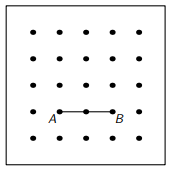
\includegraphics[scale=0.5]{geoboard.png}
\end{figure}
\item How many different values strictly between $1/2$ and 1 are obtained by computing $P/Q$ for whole numbers $P$ and $Q$ strictly between 0 and 10?\vspace{2cm}
\item (2006 National Sprint \#21) On the refrigerator, \texttt{MATHCOUNTS} is spelled out with 10 magnets, one letter per magnet. Two vowels and three consonants fall off and are put away in a bag. If the \texttt{T}s are indistinguishable, how many distinct possible collections of letters could be put in the bag?\vspace{2cm}
\item Joseph, Pedro, Samuel, and David leaves their backpacks by the classroom door. When the fire alarm rings they rush to leave, each randomly grabbing a backpack on the way out. In how many ways can the bags be taken such that each boy takes a backpack that is not his own?
\end{enumerate} 


% \newpage

% \section*{Repeated Elements}

% \begin{enumerate}
% \item If all the letters of the word $SYZYGY$\footnote{``In astronomy, a roughly straight-line configuration of three or more celestial bodies.''} are used, in how many different ways can the six letters be arranged in a six-letter string?\vspace{4cm}
% \item In how many different ways can the letters in the word $PEOPLE$ be scrambled, including the original spelling $PEOPLE$?\vspace{4cm}
% \item (2006 State Sprint Problem 28) Derek's phone number, 336-7624, has the property that the three-digit prefix, 336, equals the product of the last four digits, $7\times 6\times 2\times 4$. How many seven-digit phone numbers beginning with 336 have this property?
% \end{enumerate}


\newpage

\section*{Extensions}
\vspace{1cm}
\begin{enumerate}
\item \underline{\hspace{3in}} (2011 State Countdown)\vspace{1cm}
\item \underline{\hspace{3in}} [treat $0^0$ as undefined]\vspace{1cm}
\item \underline{\hspace{3in}} (1996 School Team)\vspace{1cm}
\item \underline{\hspace{3in}} (2012 National Sprint \#10)\vspace{1cm}
\item \underline{\hspace{3in}} (2014 State Sprint \#18)\vspace{1cm}
\item \underline{\hspace{3in}} (2012 State Sprint \#29)\vspace{1cm}
\item \underline{\hspace{3in}} (2006 National Team)
\end{enumerate}


\newpage

\section*{Extra Problems ($\star$)}

\begin{enumerate}
\item Given that $a,b,c$ are real numbers satisfying
\begin{align*}
a + b + c &= 6, \\
a^2 + b^2 + c^2 &= 20, \\
a^3 + b^3 + c^3 &= 78,
\end{align*}
find $a^4 + b^4 + c^4$.
\vspace{2cm}
\item Each of the vertices of a cube is independently colored red or blue with equal probability.
\begin{enumerate}
\item What is the expected value of the number of faces whose vertices are all the same color?
\item What is the probability that at least one face has vertices all of the same color?
\end{enumerate}
Express your answers as common fractions.
\vspace{2cm}
\item The side length of cube $ABCDEFGH$ shown below is 6. In simplest radical form, what is the shortest possible distance between a point on line $\overline{AC}$ and a point on line $\overline{BE}$?
\begin{figure}[H]
\centering
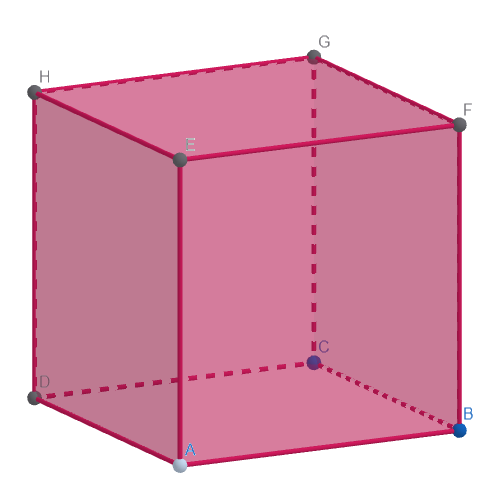
\includegraphics[scale=0.5]{cube.png}
\end{figure}
\item While 6 is the smallest possible integer area of a right triangle with integer side lengths, there are right triangles with rational side lengths of area 5. What is the smallest possible integer-valued perimeter of such a triangle?
\end{enumerate}


\end{document}